\documentclass[12pt,a4paper]{article}

\usepackage[a4paper,text={16.5cm,25.2cm},centering]{geometry}
\usepackage{lmodern}
\usepackage{amssymb,amsmath}
\usepackage{ifxetex}
\ifxetex
  \usepackage{mathspec}
\fi
\usepackage{graphics}
\usepackage{microtype}
\usepackage{hyperref}
\setlength{\parindent}{0pt}
\setlength{\parskip}{1.2ex}

\hypersetup
       {   pdfauthor = { Matti Pastell },
           pdftitle={ Intro to Weave.jl with Gadfly },
           colorlinks=TRUE,
           linkcolor=black,
           citecolor=blue,
           urlcolor=blue
       }



\title{ Intro to Weave.jl with Gadfly }



\author{ Matti Pastell }



\date{ 13th December 2016 }


\usepackage[T1]{fontenc}
\usepackage{textcomp}
\usepackage{upquote}
\usepackage{listings}
\usepackage{xcolor}
\lstset{
    basicstyle=\ttfamily\footnotesize,
    upquote=true,
    breaklines=true,
    keepspaces=true,
    showspaces=false,
    columns=fullflexible,
    showtabs=false,
    showstringspaces=false,
    escapeinside={(*@}{@*)},
    extendedchars=true,
}
\newcommand{\HLJLt}[1]{#1}
\newcommand{\HLJLw}[1]{#1}
\newcommand{\HLJLe}[1]{#1}
\newcommand{\HLJLeB}[1]{#1}
\newcommand{\HLJLo}[1]{#1}
\newcommand{\HLJLk}[1]{\textcolor[RGB]{148,91,176}{\textbf{#1}}}
\newcommand{\HLJLkc}[1]{\textcolor[RGB]{59,151,46}{\textit{#1}}}
\newcommand{\HLJLkd}[1]{\textcolor[RGB]{214,102,97}{\textit{#1}}}
\newcommand{\HLJLkn}[1]{\textcolor[RGB]{148,91,176}{\textbf{#1}}}
\newcommand{\HLJLkp}[1]{\textcolor[RGB]{148,91,176}{\textbf{#1}}}
\newcommand{\HLJLkr}[1]{\textcolor[RGB]{148,91,176}{\textbf{#1}}}
\newcommand{\HLJLkt}[1]{\textcolor[RGB]{148,91,176}{\textbf{#1}}}
\newcommand{\HLJLn}[1]{#1}
\newcommand{\HLJLna}[1]{#1}
\newcommand{\HLJLnb}[1]{#1}
\newcommand{\HLJLnbp}[1]{#1}
\newcommand{\HLJLnc}[1]{#1}
\newcommand{\HLJLncB}[1]{#1}
\newcommand{\HLJLnd}[1]{\textcolor[RGB]{214,102,97}{#1}}
\newcommand{\HLJLne}[1]{#1}
\newcommand{\HLJLneB}[1]{#1}
\newcommand{\HLJLnf}[1]{\textcolor[RGB]{66,102,213}{#1}}
\newcommand{\HLJLnfm}[1]{\textcolor[RGB]{66,102,213}{#1}}
\newcommand{\HLJLnp}[1]{#1}
\newcommand{\HLJLnl}[1]{#1}
\newcommand{\HLJLnn}[1]{#1}
\newcommand{\HLJLno}[1]{#1}
\newcommand{\HLJLnt}[1]{#1}
\newcommand{\HLJLnv}[1]{#1}
\newcommand{\HLJLnvc}[1]{#1}
\newcommand{\HLJLnvg}[1]{#1}
\newcommand{\HLJLnvi}[1]{#1}
\newcommand{\HLJLnvm}[1]{#1}
\newcommand{\HLJLl}[1]{#1}
\newcommand{\HLJLld}[1]{\textcolor[RGB]{148,91,176}{\textit{#1}}}
\newcommand{\HLJLs}[1]{\textcolor[RGB]{201,61,57}{#1}}
\newcommand{\HLJLsa}[1]{\textcolor[RGB]{201,61,57}{#1}}
\newcommand{\HLJLsb}[1]{\textcolor[RGB]{201,61,57}{#1}}
\newcommand{\HLJLsc}[1]{\textcolor[RGB]{201,61,57}{#1}}
\newcommand{\HLJLsd}[1]{\textcolor[RGB]{201,61,57}{#1}}
\newcommand{\HLJLsdB}[1]{\textcolor[RGB]{201,61,57}{#1}}
\newcommand{\HLJLsdC}[1]{\textcolor[RGB]{201,61,57}{#1}}
\newcommand{\HLJLse}[1]{\textcolor[RGB]{59,151,46}{#1}}
\newcommand{\HLJLsh}[1]{\textcolor[RGB]{201,61,57}{#1}}
\newcommand{\HLJLsi}[1]{#1}
\newcommand{\HLJLso}[1]{\textcolor[RGB]{201,61,57}{#1}}
\newcommand{\HLJLsr}[1]{\textcolor[RGB]{201,61,57}{#1}}
\newcommand{\HLJLss}[1]{\textcolor[RGB]{201,61,57}{#1}}
\newcommand{\HLJLssB}[1]{\textcolor[RGB]{201,61,57}{#1}}
\newcommand{\HLJLnB}[1]{\textcolor[RGB]{59,151,46}{#1}}
\newcommand{\HLJLnbB}[1]{\textcolor[RGB]{59,151,46}{#1}}
\newcommand{\HLJLnfB}[1]{\textcolor[RGB]{59,151,46}{#1}}
\newcommand{\HLJLnh}[1]{\textcolor[RGB]{59,151,46}{#1}}
\newcommand{\HLJLni}[1]{\textcolor[RGB]{59,151,46}{#1}}
\newcommand{\HLJLnil}[1]{\textcolor[RGB]{59,151,46}{#1}}
\newcommand{\HLJLnoB}[1]{\textcolor[RGB]{59,151,46}{#1}}
\newcommand{\HLJLoB}[1]{\textcolor[RGB]{102,102,102}{\textbf{#1}}}
\newcommand{\HLJLow}[1]{\textcolor[RGB]{102,102,102}{\textbf{#1}}}
\newcommand{\HLJLp}[1]{#1}
\newcommand{\HLJLc}[1]{\textcolor[RGB]{153,153,119}{\textit{#1}}}
\newcommand{\HLJLch}[1]{\textcolor[RGB]{153,153,119}{\textit{#1}}}
\newcommand{\HLJLcm}[1]{\textcolor[RGB]{153,153,119}{\textit{#1}}}
\newcommand{\HLJLcp}[1]{\textcolor[RGB]{153,153,119}{\textit{#1}}}
\newcommand{\HLJLcpB}[1]{\textcolor[RGB]{153,153,119}{\textit{#1}}}
\newcommand{\HLJLcs}[1]{\textcolor[RGB]{153,153,119}{\textit{#1}}}
\newcommand{\HLJLcsB}[1]{\textcolor[RGB]{153,153,119}{\textit{#1}}}
\newcommand{\HLJLg}[1]{#1}
\newcommand{\HLJLgd}[1]{#1}
\newcommand{\HLJLge}[1]{#1}
\newcommand{\HLJLgeB}[1]{#1}
\newcommand{\HLJLgh}[1]{#1}
\newcommand{\HLJLgi}[1]{#1}
\newcommand{\HLJLgo}[1]{#1}
\newcommand{\HLJLgp}[1]{#1}
\newcommand{\HLJLgs}[1]{#1}
\newcommand{\HLJLgsB}[1]{#1}
\newcommand{\HLJLgt}[1]{#1}


\begin{document}

\maketitle


This a sample \href{http://julialang.org/}{Julia} markdown document that can be executed using \href{https://github.com/mpastell/Weave.jl}{Weave.jl}.

The code is delimited from docs using markdown fenced code blocks markup which can be seen looking at the source document \href{gadfly_md_sample.jmd}{gadfly\_md\_sample.jmd} in the examples directory of the package. The source document can be executed and the results with Gadfly plots are captured in the resulting file.

You can create markdown output or pdf (with xelatex) and HTML directly using the weave command as follows:

\begin{lstlisting}
(*@\HLJLk{using}@*) (*@\HLJLn{Weave}@*)
(*@\HLJLcs{{\#}Markdown}@*)
(*@\HLJLnf{weave}@*)(*@\HLJLp{(}@*)(*@\HLJLn{Pkg}@*)(*@\HLJLoB{.}@*)(*@\HLJLnf{dir}@*)(*@\HLJLp{(}@*)(*@\HLJLs{"Weave"}@*)(*@\HLJLp{,}@*)(*@\HLJLs{"examples"}@*)(*@\HLJLp{,}@*)(*@\HLJLs{"gadfly{\_}md{\_}sample.jmd"}@*)(*@\HLJLp{),}@*) (*@\HLJLn{informat}@*)(*@\HLJLoB{=}@*)(*@\HLJLs{"markdown"}@*)(*@\HLJLp{,}@*)
  (*@\HLJLn{out{\_}path}@*) (*@\HLJLoB{=}@*) (*@\HLJLoB{:}@*)(*@\HLJLn{pwd}@*)(*@\HLJLp{,}@*) (*@\HLJLn{doctype}@*) (*@\HLJLoB{=}@*) (*@\HLJLs{"pandoc"}@*)(*@\HLJLp{)}@*)
(*@\HLJLcs{{\#}HTML}@*)
(*@\HLJLnf{weave}@*)(*@\HLJLp{(}@*)(*@\HLJLn{Pkg}@*)(*@\HLJLoB{.}@*)(*@\HLJLnf{dir}@*)(*@\HLJLp{(}@*)(*@\HLJLs{"Weave"}@*)(*@\HLJLp{,}@*)(*@\HLJLs{"examples"}@*)(*@\HLJLp{,}@*)(*@\HLJLs{"gadfly{\_}md{\_}sample.jmd"}@*)(*@\HLJLp{),}@*) (*@\HLJLn{informat}@*)(*@\HLJLoB{=}@*)(*@\HLJLs{"markdown"}@*)(*@\HLJLp{,}@*)
  (*@\HLJLn{out{\_}path}@*) (*@\HLJLoB{=}@*) (*@\HLJLoB{:}@*)(*@\HLJLn{pwd}@*)(*@\HLJLp{,}@*) (*@\HLJLn{doctype}@*) (*@\HLJLoB{=}@*) (*@\HLJLs{"md2html"}@*)(*@\HLJLp{)}@*)
(*@\HLJLcs{{\#}pdf}@*)
(*@\HLJLnf{weave}@*)(*@\HLJLp{(}@*)(*@\HLJLn{Pkg}@*)(*@\HLJLoB{.}@*)(*@\HLJLnf{dir}@*)(*@\HLJLp{(}@*)(*@\HLJLs{"Weave"}@*)(*@\HLJLp{,}@*)(*@\HLJLs{"examples"}@*)(*@\HLJLp{,}@*)(*@\HLJLs{"gadfly{\_}md{\_}sample.jmd"}@*)(*@\HLJLp{),}@*) (*@\HLJLn{informat}@*)(*@\HLJLoB{=}@*)(*@\HLJLs{"markdown"}@*)(*@\HLJLp{,}@*)
  (*@\HLJLn{out{\_}path}@*) (*@\HLJLoB{=}@*) (*@\HLJLoB{:}@*)(*@\HLJLn{pwd}@*)(*@\HLJLp{,}@*) (*@\HLJLn{doctype}@*) (*@\HLJLoB{=}@*) (*@\HLJLs{"md2pdf"}@*)(*@\HLJLp{)}@*)
\end{lstlisting}



\emph{The markdown variant used for html and pdf output is Julia markdown.}

The documents will be written to the Julia working directory when you use the \verb|out_path = :pwd|.
\subsection{Capturing code}

The basic code chunk will be run with default options and the code and output will be captured.

\begin{lstlisting}
(*@\HLJLk{using}@*) (*@\HLJLn{Gadfly}@*)
(*@\HLJLn{x}@*) (*@\HLJLoB{=}@*) (*@\HLJLnf{linspace}@*)(*@\HLJLp{(}@*)(*@\HLJLni{0}@*)(*@\HLJLp{,}@*) (*@\HLJLni{2}@*)(*@\HLJLoB{*}@*)(*@\HLJLn{pi}@*)(*@\HLJLp{)}@*)
(*@\HLJLnf{println}@*)(*@\HLJLp{(}@*)(*@\HLJLn{x}@*)(*@\HLJLp{)}@*)
\end{lstlisting}


\begin{lstlisting}
linspace(0.0,6.283185307179586,50)
\end{lstlisting}


\begin{lstlisting}
(*@\HLJLnf{plot}@*)(*@\HLJLp{(}@*)(*@\HLJLn{x}@*) (*@\HLJLoB{=}@*) (*@\HLJLn{x}@*)(*@\HLJLp{,}@*) (*@\HLJLn{y}@*) (*@\HLJLoB{=}@*) (*@\HLJLnf{sin}@*)(*@\HLJLp{(}@*)(*@\HLJLn{x}@*)(*@\HLJLp{))}@*)
\end{lstlisting}


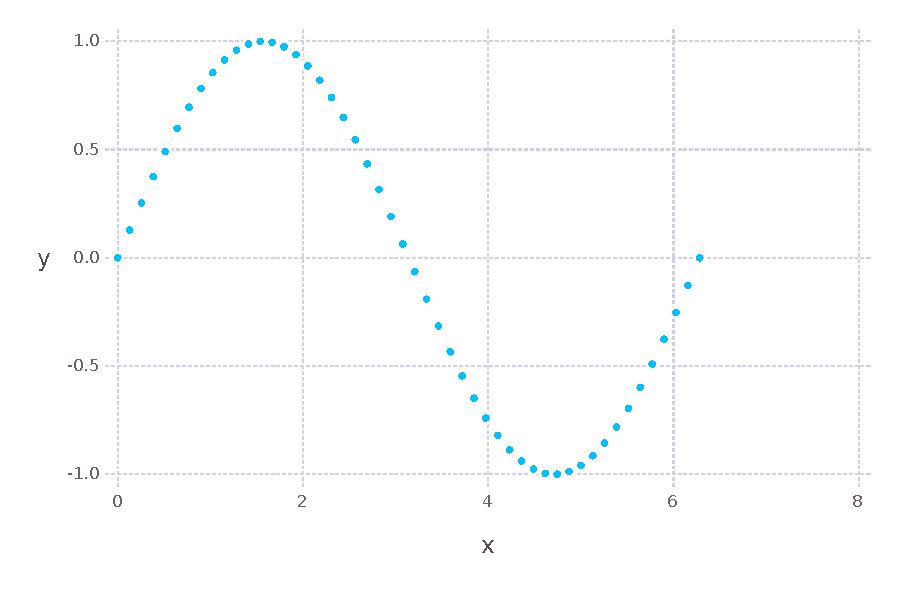
\includegraphics{figures/gadfly_md_sample_2_1.pdf}


You can also control the way the results are captured, plot size etc. using chunk options. Here is an example of a chunk that behaves like a repl.

\begin{lstlisting}
(*@\HLJLnB{julia> }@*)(*@\HLJLn{x}@*) (*@\HLJLoB{=}@*) (*@\HLJLni{1}@*)(*@\HLJLoB{:}@*)(*@\HLJLni{10}@*)

1:10
(*@\HLJLnB{julia> }@*)(*@\HLJLn{d}@*) (*@\HLJLoB{=}@*) (*@\HLJLnf{Dict}@*)(*@\HLJLp{(}@*)(*@\HLJLs{"Weave"}@*) (*@\HLJLoB{=>}@*) (*@\HLJLs{"testing"}@*)(*@\HLJLp{)}@*)

Dict{\{}String,String{\}} with 1 entry:
  "Weave" => "testing"
(*@\HLJLnB{julia> }@*)(*@\HLJLn{y}@*) (*@\HLJLoB{=}@*) (*@\HLJLp{[}@*)(*@\HLJLni{2}@*)(*@\HLJLp{,}@*) (*@\HLJLni{4}@*) (*@\HLJLp{,}@*)(*@\HLJLni{8}@*)(*@\HLJLp{]}@*)
(*@\HLJLni{3}@*)(*@\HLJLoB{-}@*)(*@\HLJLn{element}@*) (*@\HLJLnf{Array}@*)(*@\HLJLp{{\{}}@*)(*@\HLJLn{Int64}@*)(*@\HLJLp{,}@*)(*@\HLJLni{1}@*)(*@\HLJLp{{\}}}@*)(*@\HLJLoB{:}@*)
 2
 4
 8
\end{lstlisting}


You can also for instance hide the code and show only the figure, add a caption to the figure and make it wider as follows (you can only see the syntax from the source document):

\begin{figure}[!h]
\center
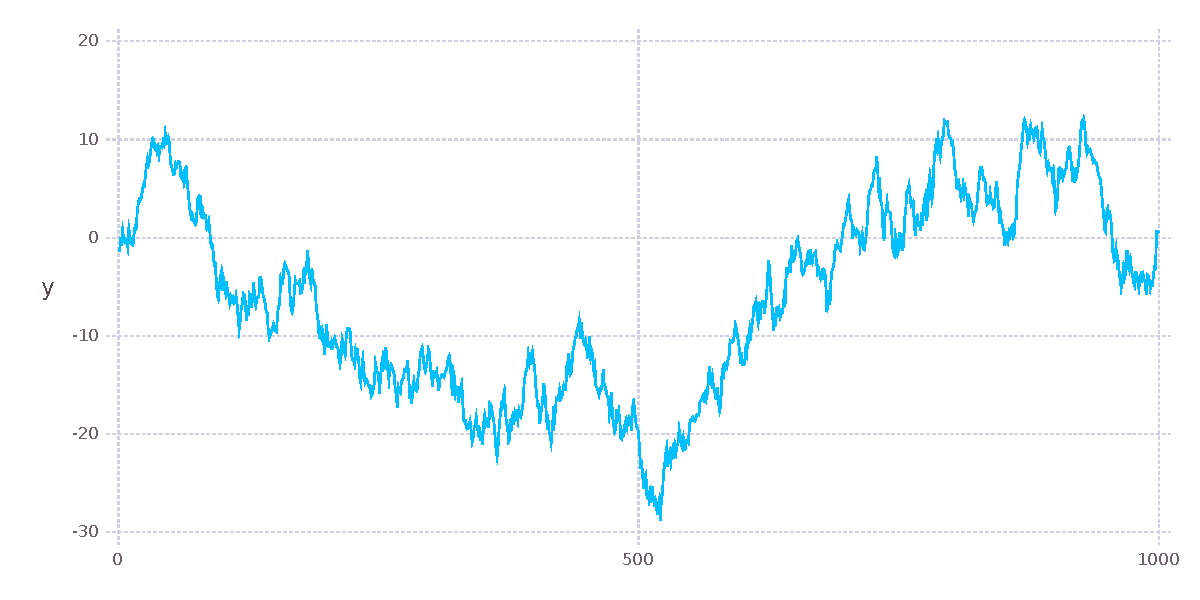
\includegraphics{figures/gadfly_md_sample_random_1.pdf}
\caption{A random walk.}
\label{fig:random}
\end{figure}

\subsection{Whats next}

Read the documentation:
\begin{itemize}
\item 
stable: \href{http://mpastell.github.io/Weave.jl/stable/}{http://mpastell.github.io/Weave.jl/stable/}

\item 
latest: \href{http://mpastell.github.io/Weave.jl/latest/}{http://mpastell.github.io/Weave.jl/latest/}
\end{itemize}

See other examples in the \href{https://github.com/mpastell/Weave.jl/tree/master/examples}{Github repo}


\end{document}
